\documentclass[12pt]{article}

\usepackage[hmargin=1in,vmargin=1in]{geometry}
\usepackage{listings}
\usepackage{color}
\usepackage{hyperref}
\usepackage{graphicx}


% For better handling of unicode (Latin characters, anyway)
\IfFileExists{lmodern.sty}{\usepackage{lmodern}}{}
\usepackage[T1]{fontenc}
\usepackage[utf8]{inputenc}

\hypersetup{
    colorlinks=true,
    linkcolor=blue,
    urlcolor=red,
    linktoc=all
}

\title{Rapport final de TIPE}
\author{PEREIRA Romain}
\date{4 Juin 2017}


\renewcommand*\contentsname{Sommaire}

\begin{document}
	\maketitle
	\tableofcontents
	
	\section*{Préambule}
		\hspace{10 mm}
		Un léger inflechissement a eu lieu quant à l'étude spatiale et temporelle de la rastérisation.
		En effet, ces problématiques me paraissent trop vastes et non appropriées pour être traitées entièrement dans le cadre de mon TIPE.
		Ainsi, j'ai décidé de me limiter à une présentation rapide du procédé dans mon étude.
		\newline
		Le reste du travail a bien été mené à son terme : j'ai étudié en détail les champs de hauteurs.


	\section{Introduction}
		\hspace{10 mm}
		Les algorithmes de rendu graphique en temps réel consistent à générer des images numériques, qui sont calculées et affichées suffisement rapidement pour faire l'illusion de continuité sur l'œil humain
		Mon travail s'est orienté sur l'étude de grille uniforme bi-dimensionnel sur-elevés, basée sur des champs de hauteurs. On peut ainsi synthétiser l'image d'un terrain rapidement grâce à une rastérisation.
		Ce TIPE décrira le processus de rendu, la façon dont on crée des champs des hauteurs, et les structures de données optimales pour les stocker en mémoire.

	\newpage
	\section{Corps principal}
		\subsection{Modalités d'action}	

		J''étudie la théorie de deux méthodes de rendus graphiques : le lancer de rayon et la rastérisation.
		Dans la synthèse d'image numérique, les objets sont souvent representés virtuellement sous forme d'une liste de vecteurs,
		qui forment un maillage surfacique de l'objet à partir de primitives géometriques (triangles, carrés, sphères...)
		 \newline
		 Je me suis naturellement interessé aux champs de hauteurs, qui sont des champs scalaires à 2 coordonnées : à une position « (x, z) » , elle associe une hauteur « y ».
		 Ils m'ont permis de génerer des surfaces de type terrain. 
		 Il m'a fallu ensuite être en mesure de triangulariser ces surfaces, afin d'en faire des objets numériques prêts à être injectés dans la rastérisation.
		\newline
		Afin de mettre en pratique ces études, j'ai crée un programme capable de travailler avec des terrains à 3 dimensions.
		J'ai ensuite utilisé une bibliothèque qui implémente le processus de rastérisation pour avoir un rendu concret.
 
		\subsection{Restitution des résultats}
			Il s'avère que pour faire de la synthèse d'image en temps réel, la rastérisation est plus adapté, je ne me suis donc pas attardé sur le lancer de rayon.
			\newline
			La complexité spatiale des champs de hauteurs m'a mené à comparer 3 méthodes de representation des données. Le résultat de cette étude est donnée ci dessous.			
			\begin{figure}[!h]
				\begin{center}
					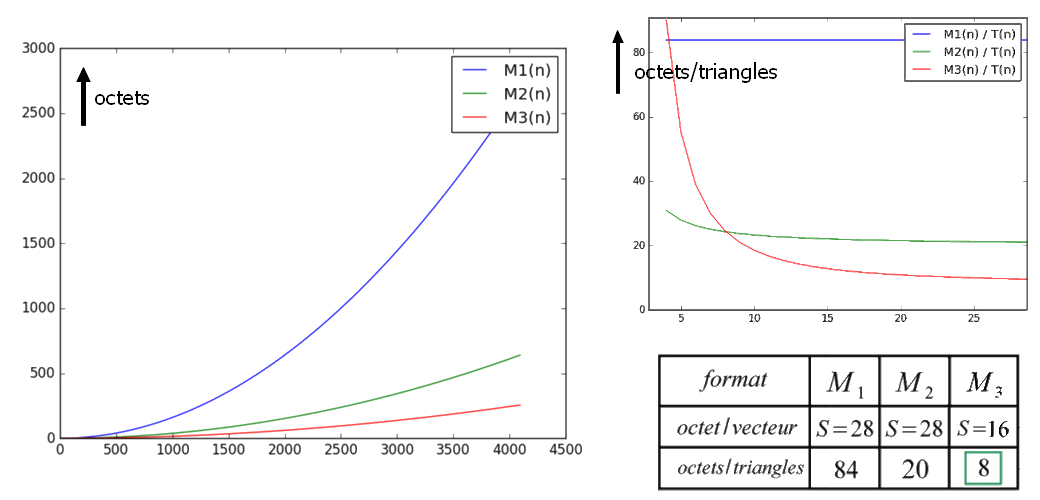
\includegraphics[width=\textwidth,height=\textheight,keepaspectratio]{../images/complexiteSpatial5.png}
				\end{center}
				\caption{\textit{Utilisation mémoire d'un terrain carré avec n vecteurs par coté}}
				\label{Utilisation mémoire du terrain}
			\end{figure}
			\newline
			J'ai decomposé l'étude de la complexité temporelle en deux sous-parties.
			\newline
			\newline
			• Il y a premièrement un temps de préparation, qui consiste à envoyer les données sur le serveur de calcul (carte graphique), et à initialiser la parallélisation.
			Ce temps dépends énormement de l'architecture du serveur (nombre de coeurs de calculs à disposition, bande passante...)
			La bande passante peut varier de 1 à 100 GO/s selon l'architecture... ce qui represente 1Mo/ms à 1Go/ms.
			Il y a ainsi un lien étroit entre les complexités spatiales et temporelles : la synthèse sera d'autant plus rapide que les données sont légères.
			\newline
			\newline
			• La deuxième sous-partie est l'execution de la rastérisation. Elle peut être interpreté comme le nombre de `triangle par secondes' que le serveur est capable de calculer.
			


		\subsection{Analyse - Exploitation - Discussion}
		J'ai cherché à optimiser l'espace mémoire requis car la complexité spatiale est très étroitement lié aux performances temporelles.
		Ainsi, j'ai pu atteindre une complexité asymptotique que je juge optimale.
		\begin{figure}[!h]
			\begin{center}
				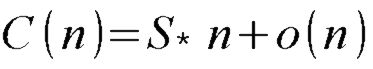
\includegraphics[height=1cm,keepaspectratio]{../images/complexity.png}
			\end{center}
			\caption{\textit{Utilisation mémoire d'un terrain carré n vecteurs (de S octets)  par coté}}
			\label{Utilisation mémoire du terrain 2}
		\end{figure}
	\newpage
	\section{Conclusion générale}
	Mon TIPE a donc été centré sur la synthèse d'image d'un terrain virtuelle, utilisant la rastérisation.
	\newline

	\newpage
	\section{Références}


\end{document}